% 01_introduction -- front lane. Numbers: \res macros; counts from juliet/full_split_v1.json (src noted inline).
\section{Introduction}
\label{sec:intro}

A memory leak (\cwe{}, ``missing release of memory after effective lifetime''~\cite{mitrecwe401}) happens when heap memory is never released.
Leaks rarely crash a program.
They show up as slow resource exhaustion in long-running services, which makes them hard to catch with tests and a natural target for static analysis.
Detectors for this bug class come in several families: path-sensitive analyzers such as the Clang Static Analyzer~\cite{clangsa}, bi-abduction and Pulse in Infer~\cite{calcagno2009biabduction,le2022pulse}, dataflow queries in CodeQL~\cite{codeqldocs}, and, more recently, large language models (LLMs) and fine-tuned classifiers.
Most of them are evaluated on the NIST Juliet C/C++ suite~\cite{boland2012juliet,sard}.
Juliet is the standard synthetic benchmark because every test case comes with a known bad and good version that compiles and runs.

Juliet generates its test cases from templates, and templates leave traces.
Before we compared any detectors, we audited the 1,658 \cwe{} groups of Juliet~v1.3 for shortcuts (\S\ref{sec:benchmark}).
The audit is sobering.
In the original files, every good unit contains a \code{static void} helper (\code{goodG2B}, \code{goodB2G}), so the rule ``\code{static void} $\Rightarrow$ good'' reaches macro-F1 \res{x}{probe_static_void_original}.
A one-line grep rule, ``no \code{free}/\code{delete} $\Rightarrow$ leak'', reaches \res{grep-original}{macro}.
That is higher than Clang SA (\res{clang_sa-original}{macro}), CodeQL (\res{codeql-original}{macro}) and Infer (\res{infer-original}{macro}) on the same units (Table~\ref{tab:orig}).
On original Juliet, a high score therefore says little about whether a detector reads the code.
Germano et al.\ report similar template biases in Juliet for machine-learning detectors~\cite{germano2025biased}.
Risse and B\"ohme show the same problem for real-world vulnerability datasets~\cite{risse2024limits,risse2025topscore}.

We therefore rebuild the benchmark before using it (Fig.~\ref{fig:overview}).
\Deb{} keeps one entry point per unit, removes \code{static}, comments and Juliet identifiers, and uses the same driver for both labels.
Every label is checked by compilation and by LeakSanitizer.
\Dead{} adds frees that can never execute; a detector that only looks for a \code{free} call now sees a ``fix'' in every bad unit.
\Plac{} adds never-executed print statements at the same places, so we can tell whether a detector reacts to the dead frees or only to the edit.
We split by flow variant rather than by family, so a held-out variant tests a control-flow shape that no trained model has seen.
On these layers we compare static analyzers, two LLMs with four prompting strategies, two off-the-shelf decision models, a LoRA decision model that we fine-tune on Juliet, LineVul, and the grep rule.
Sanitizers and Valgrind serve as a dynamic reference.

\begin{figure}[t]
\centering
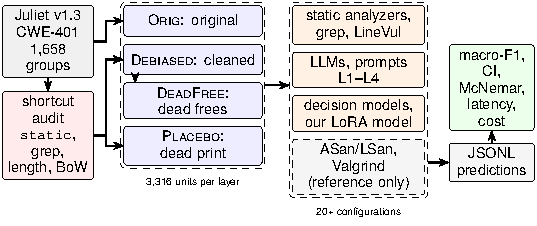
\includegraphics[width=\columnwidth]{figures_front/overview.pdf}
\caption{Study overview. We audit the \cwe{} part of Juliet for shortcuts, rebuild it into \Deb{} with two controlled variants (\Dead, \Plac), keep \Orig{} for comparison, and score all detectors from one prediction format.}
\label{fig:overview}
\end{figure}

We answer four research questions:
\begin{itemize}
\item \textbf{RQ1 (benchmark validity):} Can trivial shortcuts solve original Juliet \cwe{}, and does our debiasing remove them?
\item \textbf{RQ2 (approaches):} How do prompting strategies L1--L4, decision models and static analyzers compare on \Deb?
\item \textbf{RQ3 (efficiency):} Which accuracy--latency--cost trade-offs suit IDE, pre-commit and CI use?
\item \textbf{RQ4 (robustness):} Do detectors reason about path feasibility when never-executed frees are added (\Dead, controlled by \Plac)? Does fine-tuning amplify shortcuts?
\end{itemize}

\noindent Our contributions are:
\begin{enumerate}
\item A shortcut audit of Juliet \cwe{}: format, length, grep and bag-of-words probes, measured on every layer (Table~\ref{tab:probes}).
\item A debiased \cwe{} benchmark of 3,316 label-verified units, plus a dead-free stress layer and a placebo control, with a flow-variant split. % src: juliet/full_split_v1.json
\item A unified comparison of more than 20 detector configurations on accuracy, latency and cost, all scored by the same pipeline.
\item Findings that a template-free benchmark exposes, summarized below.
\end{enumerate}

\noindent\textbf{Summary of findings.}
On \Deb{} the probes fall to chance (\code{static void} \res{x}{probe_static_void_layer1}, length \res{x}{probe_length_lines_layer1}), and the grep rule falls to \res{grep-layer1}{macro}.
Clang SA and Infer give the same score on \Deb, \Dead{} and \Plac{}: their change on \Dead{} is \res{clang_sa-layer3}{d} and \res{infer-layer3}{d}, respectively.
LLMs and decision models fail in two opposite ways on \Dead.
Some treat any \code{free} as a fix.
Our fine-tuned model is the extreme case: its recall falls to \res{lora_L1-layer3}{r} although it scores \res{lora_L1-layer1}{macro} on \Deb, so fine-tuning learned the shortcut.
Others treat dead frees as suspicious: Qwen3.5-4B L1 adds \res{qwen_L1-layer3}{gained} new false alarms.
Jev changes least among learned detectors (\res{jev_L1-layer3}{d}).
Among prompting strategies, L4 (LLM-extracted facts and a Datalog rule) loses least for both LLMs (\res{deepseek_L4-layer3}{d} and \res{qwen_L4-layer3}{d}).

The rest of the paper is organized as follows.
\S\ref{sec:background} gives background.
\S\ref{sec:benchmark} builds the benchmark.
\S\ref{sec:methods} describes the detectors and the setup.
\S\ref{sec:results} and \S\ref{sec:discussion} report and discuss results.
\S\ref{sec:threats} lists threats to validity.
